\documentclass[tikz,border=4pt]{standalone}
\usepackage{amsmath}
\begin{document}
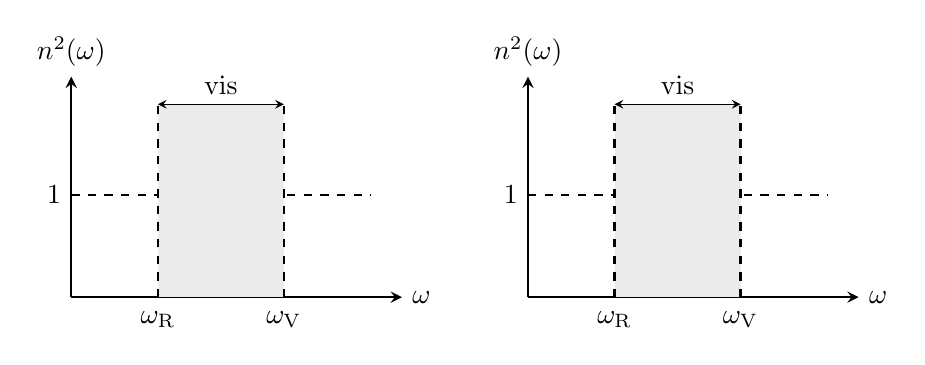
\begin{tikzpicture}[>=stealth, thick, scale=1.0]
  % Left: Quartz template
  \begin{scope}[xshift=0cm]
    \draw[->] (0, 0) -- (4.2, 0) node[right] {$\omega$};
    \draw[->] (0, 0) -- (0, 2.8) node[above] {$n^2(\omega)$};
    \draw[dashed] (0, 1.3) -- (3.8, 1.3);
    \node[left] at (0, 1.3) {$1$};

    % Visible region
    \fill[black!8] (1.1, 0) rectangle (2.7, 2.45);
    \draw[dashed] (1.1, 0) -- (1.1, 2.45);
    \draw[dashed] (2.7, 0) -- (2.7, 2.45);
    \draw[<->, thin] (1.1, 2.45) -- (2.7, 2.45) node[midway, above] {$\mathrm{vis}$};
    \node[below] at (1.1, -0.05) {$\omega_{\mathrm{R}}$};
    \node[below] at (2.7, -0.05) {$\omega_{\mathrm{V}}$};
  \end{scope}

  % Right: Substance F template
  \begin{scope}[xshift=5.8cm]
    \draw[->] (0, 0) -- (4.2, 0) node[right] {$\omega$};
    \draw[->] (0, 0) -- (0, 2.8) node[above] {$n^2(\omega)$};
    \draw[dashed] (0, 1.3) -- (3.8, 1.3);
    \node[left] at (0, 1.3) {$1$};

    % Visible region
    \fill[black!8] (1.1, 0) rectangle (2.7, 2.45);
    \draw[dashed] (1.1, 0) -- (1.1, 2.45);
    \draw[dashed] (2.7, 0) -- (2.7, 2.45);
    \draw[<->, thin] (1.1, 2.45) -- (2.7, 2.45) node[midway, above] {$\mathrm{vis}$};
    \node[below] at (1.1, -0.05) {$\omega_{\mathrm{R}}$};
    \node[below] at (2.7, -0.05) {$\omega_{\mathrm{V}}$};
  \end{scope}
\end{tikzpicture}
\end{document}
